\documentclass{ximera}

\newcommand{\dfn}{\textbf}
\renewcommand{\vec}[1]{{\overset{\boldsymbol{\rightharpoonup}}{\mathbf{#1}}}\hspace{0in}}
%% Simple horiz vectors
\renewcommand{\vector}[1]{\left\langle #1\right\rangle}
\newcommand{\arrowvec}[1]{{\overset{\rightharpoonup}{#1}}}
\newcommand{\R}{\mathbb{R}}
\newcommand{\transpose}{\intercal}
\newcommand{\ro}{\texttt{R}}%% row operation
\newcommand{\dotp}{\bullet}%% dot product

\usetikzlibrary{calc,bending}
\tikzset{>=stealth}


\usepackage{mdframed} % For framing content
%\usepackage{ifthen}   % For conditional statements

% Define the 'concept' environment with an optional header
\newenvironment{concept}[1][]{%
  \begin{mdframed}[linecolor=black, linewidth=2pt, innertopmargin=5pt, innerbottommargin=5pt, skipabove=12pt, skipbelow=12pt]%
    \noindent\large\textbf{#1}\normalsize%
}{%
  \end{mdframed}%
}











%% \colorlet{textColor}{black}
%% \colorlet{background}{white}
%% \colorlet{penColor}{blue!50!black} % Color of a curve in a plot
%% \colorlet{penColor2}{red!50!black}% Color of a curve in a plot
%% \colorlet{penColor3}{red!50!blue} % Color of a curve in a plot
%% \colorlet{penColor4}{green!50!black} % Color of a curve in a plot
%% \colorlet{penColor5}{orange!80!black} % Color of a curve in a plot
%% \colorlet{penColor6}{yellow!70!black} % Color of a curve in a plot
%% \colorlet{fill1}{penColor!20} % Color of fill in a plot
%% \colorlet{fill2}{penColor2!20} % Color of fill in a plot
%% \colorlet{fillp}{fill1} % Color of positive area
%% \colorlet{filln}{penColor2!20} % Color of negative area
%% \colorlet{fill3}{penColor3!20} % Fill
%% \colorlet{fill4}{penColor4!20} % Fill
%% \colorlet{fill5}{penColor5!20} % Fill
%% \colorlet{gridColor}{gray!50} % Color of grid in a plot


\author{Bart Snapp \and Parisa Fatheddin \and Tae Eun Kim}
%%OpenAI. (2023). ChatGPT (Mar 14 version) [Large language model]. https://chat.openai.com/chat

\title{Vectors and scalars}

\begin{document}
\begin{abstract}
  A concrete introduction to vectors along with some examples of real world applications.
\end{abstract}
\maketitle


\begin{quote}
  Isn’t it time that these most ancient sorrows of ours grew fruitful?
  Time that we tenderly loosed ourselves from the loved one, and,
  unsteadily, survived: the way the arrow, suddenly all vector,
  survives the string to be more than itself.



  \hfill ---R.M.\ Rilke
\end{quote}


In mathematics, we study (among other things) numbers. In many cases,
these numbers represent real-world data. Sometimes it ``makes sense''
to add data and sometimes it doesn't.
\begin{concept}[When it does NOT make sense to add data]
\begin{description}
\item[Personal Identification Numbers] Summing things like social
  security numbers, phone numbers, or zip codes doesn't provide
  meaningful information.
\item[Temperatures] While you can mathematically add temperatures
  together, doing so usually doesn't provide useful information.
\item[Time] Adding specific points in time, like dates or hours of the
  day, usually doesn't yield meaningful results.
\item[Geographic Coordinates] Adding the latitude and longitude of two
  locations doesn't give you a location that has any real-world
  significance.
\end{description}
\end{concept}
For some of the categories above, the \textit{average} can be
meaningful or perhaps if each quantity is thought of as `displacement'
or `duration,' summing might be meaningful. However, without
\textbf{addition}al (pun intended!) stipulations, summing the types of
quantities above is not meaningful. On the other hand, there are lots
of times that it makes sense to add data. Data is represented by a
\textit{vector} when it is reasonable to add separate data points.

\begin{concept}[When it makes sense to add data]
\begin{description}
\item[Population Counts] Adding the populations of different regions,
  cities, or countries to find the total population of a larger
  area. Answers to questions like these help us understand our
  society and in turn, aid our future decisions.
\item[Consumer Data] The number of distinct products that are bought
  by a given consumer can be encoded as a vector. Summing data like
  this will tell us the total number of products purchased by a group of consumers.
%% \item[Financial Transactions] Summing daily sales to find total
%%   monthly sales, or adding up all expenses to find total costs. These
%%   are real numbers that represent actual amounts of money, and their
%%   total gives meaningful information about financial status or
%%   performance.
%% \item[Time Spent on Tasks] Adding the duration of time spent on
%%   various activities on day gives a total time spent. We all have busy
%%   lives, and time is a very precious commodity. Hence, it is good to
%%   understand how we spend our time.
\item[RGB Color Space] Colors on digital screens are often represented
  as vectors in the \link[RGB color space]{https://en.wikipedia.org/wiki/RGB_color_model}:
  \begin{center}
    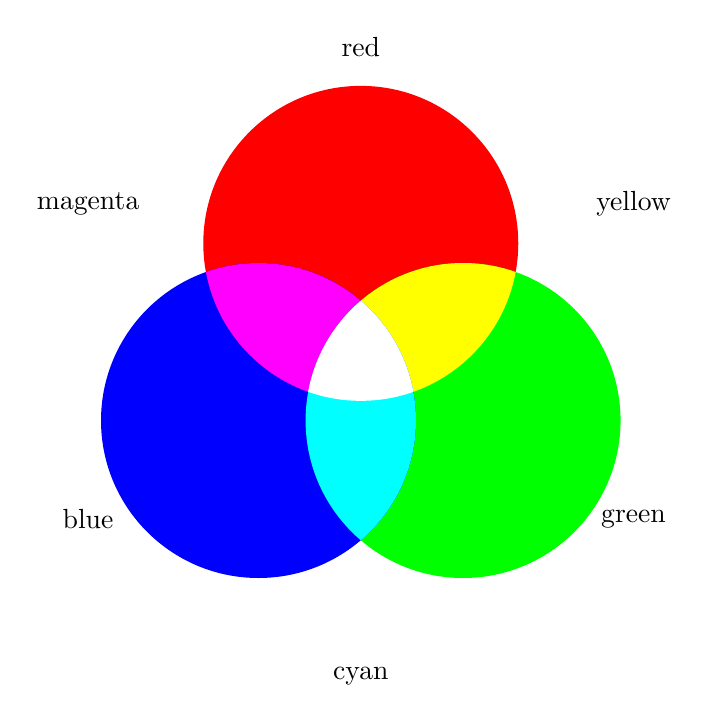
\begin{tikzpicture}%%https://texample.net/tikz/examples/rgb-color-mixing/
      \definecolor{rgbred}{RGB}{255,0,0}
      \definecolor{rgbgreen}{RGB}{0,255,0}
      \definecolor{rgbblue}{RGB}{0,0,255}
      \definecolor{rgbyellow}{RGB}{255,255,0}
      \definecolor{rgbcyan}{RGB}{0,255,255}
      \definecolor{rgbmagenta}{RGB}{255,0,255}
% On top of the background draw three spotlights of the primary colors
% red, green and blue (they are primary in an additive colorspace where
% light are mixed)
\draw [draw=none, fill=rgbred] (90:1.5) circle (2cm);
\draw [draw=none, fill=rgbgreen] (-30:1.5) circle (2cm);
\draw [draw=none, fill=rgbblue] (210:1.5) circle (2cm);

% Draw areas where two of the three primary colors are overlapping.
% These areas are the secondary colors yellow, cyan and magenta.
\begin{scope} % red + green = yellow
	\clip (90:1.5) circle(2cm);
	\draw [draw=none, fill=rgbyellow] (-30:1.5) circle (2cm);
\end{scope} % blue + red = magenta
\begin{scope}
	\clip (210:1.5) circle(2cm);
	\draw [draw=none, fill=rgbmagenta] (90:1.5) circle (2cm);
\end{scope}
\begin{scope} % green + blue = cyan
	\clip (-30:1.5) circle(2cm);
	\draw [draw=none, fill=rgbcyan] (210:1.5) circle (2cm);
\end{scope}

% Draw the center area which consists of all the primary colors.
\begin{scope} % red + green + blue = white
	\clip (90:1.5) circle(2cm);
	\clip (210:1.5) circle(2cm);
	\draw [draw=none, fill=white] (-30:1.5) circle (2cm);
\end{scope}

\foreach \x/\text in {0/red, 60/yellow, 120/green, 180/cyan, 240/blue, 300/magenta}
	\draw (-\x+90:4) node {\text};
\end{tikzpicture}
  \end{center}
  Here, three numerical components correspond to the intensity of red,
  green, and blue light, with $0$ representing no intensity and $255$
  representing the maximum intensity of the colors. Hence the color
  black can be represented by $(0,0,0)$ and white is represented by
  $(255,255,255)$.  Adding the values for different pixels changes the
  brightness of each individual component.
\item[Navigation] Aircraft navigate by knowing the direction and speed
  at which they are traveling. When interpreted correctly, this data
  can be added to help model and understand the speed and direction of
  many different ``course changes.'' Practically, this helps to find
  the ultimate position of the aircraft.
\end{description}
\end{concept}



\section{Vectors, adding and scaling}


Often when it makes sense to \textit{add} quantities, it also makes
sense to \textit{scale} them. For example, if we consider the
populations of cities, say Columbus, Ohio; Minneapolis, Minnesota; and
Chicago, Illinois, it is meaningful to say things like
\begin{itemize}
\item The population of Minneapolis is \textit{half-of} the population of Columbus.
\item The population of Chicago is \textit{three times} the population of Columbus.
\end{itemize}
In a similar way, \textit{scaling} makes sense for the other examples
above: Consumer Data, RGB Color Space, and Navigation. When
we ``scale'' vectors (data) by numbers, we call those ``scaling'' numbers
\textit{scalars}.

\begin{definition}
  We say data is represented by \dfn{vectors} $\vec{v}$ and $\vec{w}$
  if
  \[
  \vec{v}+\vec{w}
  \]
  is also a vector, encoding `meaningful' data in the same way that
  $\vec{v}$ and $\vec{w}$ do, and for all \textbf{scalars} $s$, where
  $s$ is usually a real number,
  \[
  s(\vec{v} + \vec{w}) = s\vec{v}+ s\vec{w}.
  \]
  again represents `meaningful' data in the same way that $\vec{v}$
  and $\vec{w}$ do.
\end{definition}

These informal definitions of vectors and scalars in fact contain the
\textit{essence} of the concept of a \textit{vector space}. If this
seems too abstract, I assure you that we will be giving concrete
examples along the way. At this point we need to give some notation
for vectors.

\begin{concept}[Ways data can be stored as a vector]
\begin{description}
\item[Ordered tuple] An ordered pair is just a pair of numbers
  $(a,b)$ delineated by parenthesis with the entries separated by a
  comma. It's called ``ordered'' because $(a,b) \ne (b,a)$. An \textit{ordered
  tuple} is just a list of an arbitrary, but fixed, number of elements
  that is ordered like an ordered pair. As an example, we could
  represent the \link[demographic information]{https://worldpopulationreview.com/states/states-by-race} for Ohio as an vector
  represented by an ordered tuple:
  \[
  \vec{p}_{\texttt{OH}} = (\underset{\text{White}}{9394878},\underset{\begin{smallmatrix}\text{African}\\ \text{American}\end{smallmatrix}}{1442655},\underset{\begin{smallmatrix}\text{Native}\\\text{American}\end{smallmatrix}}{20442},\underset{\text{Asian}}{268527},\underset{\text{Hawaiian}}{3907},\underset{\text{Other}}{544866})
  \]
\item[Row vector] A row vector is a lot like an ordered tuple, except
  we do not use a comma to separate entries. Instead, we separate them
  by some space.  Suppose a streaming service records the number of
  times each consumer has watched a video as a row vector. For
  example, for the $1729$th consumer, their data might look like
  \[
  \vec c_{1729} = \begin{pmatrix} 1 & 4 & 0 & \cdots & 2 & 0 \end{pmatrix}
  \]
  The different entries represent the number of times this consumer
  has watched various videos.
  \item[Column vector] A column vector is just like a row vector,
  except is it written vertically:
  \[
  \vec{p} = \begin{pmatrix}
    159\\  226 \\ 191\end{pmatrix}
    \qquad
    \begin{array}{l}
    \text{Red}\\
    \text{Green}\\
    \text{Blue}
    \end{array}
  \]
  Above, we suppose that $\vec{p}$ represents the color that
  represents the color \textit{Sea Foam Green}. Here we see the color in all of its glory:
  \begin{center}
    \colorbox[RGB]{159, 226, 191}{
      \parbox{1cm}{\rule{0pt}{1cm}}}
  \end{center}
  %% \item[As a column vector] A column vector is just like a row vector,
%%   except is it written vertically:
%%   \[
%%   \vec{w}_{\texttt{TR}} = \begin{pmatrix}
%%     0.5\\ 4 \\ 0 \\ 1\end{pmatrix}
%%     \qquad
%%     \begin{array}{l}
%%     \text{Emails}\\
%%     \text{Classes}\\
%%     \text{Projects}\\
%%     \text{Exercising}
%%   \end{array}
%%   \]
%%   Above, we could suppose that $\vec{w}_{\texttt{TR}}$ represents the
%%   fact that on Tuesdays and Thursdays, someone spends $0.5$ hours on
%%   emails, $4$ hours in class, $0$ hours on projects, and $1$ hour
%%   exercising.
\end{description}
\end{concept}

Of course, since mathematics is a human endeavor you will find
variations on the notations above. For instance, some folks use
different brackets like these
\[
\langle a, b, c \rangle, \quad \begin{bmatrix} a & b & c \end{bmatrix}, \quad
\begin{bmatrix}
  a\\
  b\\
  c
\end{bmatrix}
\]
for ordered-tuple vectors, row vectors, and column vectors,
respectively. Ordered tuples and row vectors are easy to write in-line
(in a sentence), because they are horizontal. On the other hand,
column vectors take up less horizontal space and are more convenient
when you have vectors with many entries.


\begin{definition}
  To convert a row vector to a column vector and vice versa, we use
  the \dfn{transpose} operation:
  \[
  \begin{pmatrix} 1 &  2 & 3 \end{pmatrix}^\transpose =
  \begin{pmatrix} 1 \\ 2 \\ 3 \end{pmatrix}
  \quad\text{and}\quad
  \begin{pmatrix} 1 \\ 2 \\ 3 \end{pmatrix}^\transpose =
  \begin{pmatrix} 1 &  2 & 3 \end{pmatrix}
  \]
  We read the above as ``the transpose of the row (or column) vector $1$,
  $2$, $3$ is the column (or row) vector $1$, $2$, $3$,'' respectively.
\end{definition}


\begin{question}
  Let
  $\vec{s} = \begin{pmatrix}141 & 304 & 249 & 199 &
    251 \end{pmatrix}$. Find $\vec{s}^\transpose$.
  \begin{prompt}
  \[
  \vec{s}^\transpose  = \begin{pmatrix}\answer{141} \\ \answer{304} \\ \answer{249} \\ \answer{199} \\ \answer{251} \end{pmatrix}
  \]
  \end{prompt}
\end{question}

Once we have data represented as vectors encoded as ordered tuples,
row vectors, or column vectors, we can describe some general
information about these vectors. In particular, we can consider their
\textit{length} and their \textit{components}.

\begin{definition}
  The \dfn{length} of a vector is the number of entries.  A vector of
  length $n$ can be called an \dfn{$\boldsymbol{n}$-vector}.
  % $\boldsymbol n$\textbf{-vector}
  Each individual entry of a vector is called a \dfn{component}. The
  set of all $n$-vectors of real entries is called the \dfn{Euclidean
    $\boldsymbol{n}-space$} and is denoted by $\mathbb{R}^n$.
\end{definition}

\begin{question}
  What is the length of the vector $\vec{p}_{\texttt{OH}}$?
  \begin{prompt}
  \[
  \text{Length} = \answer{6}
  \]
  \end{prompt}
\end{question}
When we express vectors as ordered tuples, row vectors, or column
vectors we add them in a componentwise fashion.
\begin{align*}
  (1,2,3) + (4,5,6) &= (5,7,9)\\
  \begin{pmatrix} 1 & 2 & 3   \end{pmatrix} + \begin{pmatrix} 4 & 5 & 6   \end{pmatrix}&= \begin{pmatrix} 5 & 7 & 9   \end{pmatrix}\\
  \begin{pmatrix} 1\\ 2\\ 3   \end{pmatrix} + \begin{pmatrix} 4\\ 5\\ 6   \end{pmatrix} &= \begin{pmatrix} 5\\ 7\\ 9   \end{pmatrix}
\end{align*}
\begin{warning}
  We may only add two vectors if they have the same length.
\end{warning}




We can also multiply vectors by a \dfn{scalar} (a number), by
multiplying each component by the scalar.
\begin{align*}
  5\cdot   (1,2,3) &= (5,10,15)\\
  5\cdot \begin{pmatrix} 1 & 2 & 3   \end{pmatrix}  &= \begin{pmatrix} 5 & 10 & 15   \end{pmatrix}\\
  5\cdot  \begin{pmatrix} 1\\ 2\\ 3   \end{pmatrix} &= \begin{pmatrix} 5\\ 10\\ 15   \end{pmatrix}
\end{align*}
Now that we know the basics, onto the examples!


\begin{example}[Population Counts] %https://worldpopulationreview.com/states/states-by-race
  The Midwest of the United States consists of $12$ states. We can
  express the $2023$
  \link[demographics]{https://worldpopulationreview.com/states/states-by-race}
  of each state as a vector represented by an ordered tuple. The
  ordered tuple for Ohio looks like:
  \[
  \vec{p}_{\texttt{OH}} = (\underset{\text{White}}{9394878},\underset{\begin{smallmatrix}\text{African}\\ \text{American}\end{smallmatrix}}{1442655},\underset{\begin{smallmatrix}\text{Native}\\\text{American}\end{smallmatrix}}{20442},\underset{\text{Asian}}{268527},\underset{\text{Hawaiian}}{3907},\underset{\text{Other}}{544866}).
  \]
  The ordered tuples for each state in the Midwest looks like:
\begin{align*}
  \vec{p}_{\texttt{IA}} &= (2806418,117035,10538,79296,3941,132783)\\
  \vec{p}_{\texttt{IL}} &= (8874067,1796660,33972,709567,5196,1296702)\\
  \vec{p}_{\texttt{IN}} &= (5510354,631923,14030,158705,2205,379676)\\
  \vec{p}_{\texttt{KA}} &= (2416165,165837,22278,87093,2344,218902)\\
  \vec{p}_{\texttt{MI}} &= (7735902,1360149,50035,316844,3117,507860)\\
  \vec{p}_{\texttt{MN}} &= (4572149,359817,54558,275242,2201,336199)\\
  \vec{p}_{\texttt{MO}} &= (4978046,698043,24274,123810,8887,291100)\\
  \vec{p}_{\texttt{ND}} &= (651470,23959,39165,11979,1004,32817)\\
  \vec{p}_{\texttt{NE}} &= (1641256,91896,16875,47944,1235,124620)\\
  \vec{p}_{\texttt{OH}} &= (9394878,1442655,20442,268527,3907,544866)\\
  \vec{p}_{\texttt{SD}} &= (735228,18836,74975,12413,544,37340)\\
  \vec{p}_{\texttt{WI}} &= (4895065,367889,48674,163396,2672,329279)
\end{align*}
\begin{enumerate}
\item What are the combined demographics of the states Michigan, Ohio,
  and Indiana?
\item Suppose that the annual percentage growth rate of Ohio is
  currently $0.1\%$. Assuming this is even across all demographics,
  what might the population data look like for Ohio in $2025$?
\end{enumerate}
\begin{explanation}
  We'll use the properties of vectors to solve this problem.
  \begin{enumerate}
  \item To find the combined demographics of Michigan, Ohio, and
    Indiana we compute
    \[
    \vec{p}_{\texttt{MI}} + \vec{p}_{\texttt{OH}} + \vec{p}_{\texttt{IN}} = \left(\answer[given]{22641134},\answer[given]{3434727},\answer[given]{84507},744076,9229,1432402\right).
    \]
  \item To find the population demographics of Ohio in \textit{two}
    years, we use the scalar, $1.001^2$, to find:
    \[
      1.001^2 \vec{p}_{\texttt{OH}}
      =\left(\answer[given]{9413677},\answer[given]{1445542},\answer[given]{20483},269064,3915,545956
      \right).
    \]
    % \[
    % 1.001 \vec{p}_{\texttt{OH}} =\left(\answer[given]{9404273},\answer[given]{1444098},\answer[given]{20462},268796,3911,545411 \right)
    % \]
  \end{enumerate}
\end{explanation}
\end{example}


\begin{example}[Consumer Data]
  The \textit{MOOCulus Streaming Service} is studying their top $5$
  most popular videos for their top $2000$ consumers. They encode this
  data as row vectors with the entries running from the most popular
  to the least. We denote these by $\vec c_1, \dots, \vec
  c_{2000}$. The vector encodes how many time each consumer has
  watched each video. For example, for the $1729$th consumer, their
  data might look like
  \[
  \vec c_{1729} = \begin{pmatrix} 1 & 4 & 0 &  2 & 0 \end{pmatrix}.
  \]
  \begin{enumerate}
  \item Interpret this vector in this context.
  \item Interpret the sum of the vectors $\vec{c}_1, \dots,
    \vec{c}_{2000}$.
  \end{enumerate}
  \begin{explanation}
    We'll answer these in turn.
    \begin{enumerate}
    \item In this context, we see that the viewer has watched the most
      popular movie $\answer[given]{1}$ time, the next most popular
      movie $\answer[given]{4}$ times, the third most popular movie
      $\answer[given]{0}$ times, and has seen the last two movies
      $\answer[given]{2}$ and zero times, respectively.
    \item The sum of the vectors $\vec{c}_1, \dots, \vec{c}_{2000}$
      represents the total number of views of the five most popular
      videos.
    \end{enumerate}
  \end{explanation}
\end{example}


%% \begin{example}[Financial Transactions]
%%   A bookstore sells a variety of books. We'll express the number of
%%   each type of book sold in one month as a row vector
%%   \[
%%   \vec{s} = \begin{pmatrix}141 & 304 & 249 & 199 & 251 \end{pmatrix}
%%   \]
%%   with the entries representing the categories: Science Fiction,
%%   Fantasy, Mystery, Romance, History in that order.  If each book
%%   costs the bookstore $6$ dollars from the wholesaler, and each book sells
%%   for $9$ dollars, what is the profit for each category?
%%   \begin{explanation}
%%     Using the properties of vectors, we wish to compute:
%%     \[
%%     9\vec{s}-6\vec{s} = \begin{pmatrix} \answer[given]{423} & \answer[given]{912} & \answer[given]{747} & 597 & 753 \end{pmatrix}
%%     \]
%%   \end{explanation}
%% \end{example}


\begin{example}[RGB Color Space]
  The \textit{MOOCulus Lighting Company} has designed an LED table
  lamp whose shades vary linearly, at a constant rate, through six
  colors ($3$ primary and $3$ secondary) of the RGB color space in
  this order:
    \[
    \underset{\text{red}}{\begin{pmatrix}255\\0\\0\end{pmatrix}},\;
    \underset{\text{yellow}}{\begin{pmatrix}255\\255\\0\end{pmatrix}},\;
    \underset{\text{green}}{\begin{pmatrix}0\\255\\0\end{pmatrix}},\;
    \underset{\text{cyan}}{\begin{pmatrix}0\\255\\255\end{pmatrix}},\;
    \underset{\text{blue}}{\begin{pmatrix}0\\0\\255\end{pmatrix}},\;
    \underset{\text{magenta}}{\begin{pmatrix}255\\0\\255\end{pmatrix}}.
    \]
    Here are the actual colors:
    \begin{center}
      
\begin{tikzpicture}
        \definecolor{rgbyellow}{RGB}{255,255,0}
        \definecolor{rgbcyan}{RGB}{0,255,255}
        \definecolor{rgbmagenta}{RGB}{255,0,255}
        \fill[fill=red] (0,0) rectangle (1,1);
        \fill[fill=rgbyellow] (1,0) rectangle (2,1);
        \fill[fill=green] (2,0) rectangle (3,1);
        \fill[fill=rgbcyan] (3,0) rectangle (4,1);
        \fill[fill=blue] (4,0) rectangle (5,1);
        \fill[fill=rgbmagenta] (5,0) rectangle (6,1);
      \end{tikzpicture}
    \end{center}
  If the lamp is turned on, it initially shows red, then this fades to
  yellow after one minute, then fades to green after a minute more,
  and so on. After $6$ minutes it is back to red. Color $\vec{c}_1$
  fades to $\vec{c}_2$ like the vector function $\vec{f}(t)$
  \[
  \vec{f}(t) = \vec{c}_1+ t(\vec{c}_2 -\vec{c}_1)
  \]
  as $t$ runs from $0$ to $1$. Note $\vec{f}(0) = \vec{c}_1$ and
  $\vec{f}(1) = \vec{c}_2$.  What RGB color is the lamp showing at $4$
  minutes and $40$ seconds?
  \begin{explanation}
    At $4$ minutes and $40$ seconds, our lamp is showing some color
    between blue and magenta. Let
    \[
      \vec{c}_1 = \begin{pmatrix}0\\0\\255\end{pmatrix} \quad\text{and}\quad
      \vec{c}_2 = \begin{pmatrix}255\\0\\255\end{pmatrix}.
    \]
    Since $40$ seconds is $2/3$ of a minute, we write
    \begin{align*}
      \vec{f}(2/3) &= \vec{c}_{1}+ \left(\answer[given]{2/3}\right)(\vec{c}_2 -\vec{c}_1) \\
      &= \begin{pmatrix}0\\0\\255\end{pmatrix}+ \left(\answer[given]{2/3}\right)\left(\begin{pmatrix}255\\0\\255\end{pmatrix}  -  \begin{pmatrix}0\\0\\255\end{pmatrix}\right) \\
      &=\begin{pmatrix}0\\0\\255\end{pmatrix}+ \left(\answer[given]{2/3}\right)\begin{pmatrix}255\\0\\0\end{pmatrix} \\
                &=\begin{pmatrix}170\\0\\255\end{pmatrix}.
    \end{align*}
    Here is this color:
    \begin{center}
    \colorbox[RGB]{170,0, 255}{
      \parbox{1cm}{\rule{0pt}{1cm}}}
  \end{center}
  \end{explanation}
\end{example}





%% \begin{example}[Time Spent on Tasks]
%%   On Mondays, Wednesdays, and Fridays, suppose you spend you spend $1$
%%   hour on emails, $2$ hours in class, and $3$ hours working on
%%   projects. On Tuesdays and Thursdays, you spend $1/2$ hour on emails,
%%   $4$ hours in class, and $1$ hour exercising. We can express each day
%%   as a column vector:
%%   \[
%%   \vec{w}_{\texttt{MWF}} =
%%   \begin{pmatrix}
%%     1 \\
%%     2 \\
%%     3 \\
%%     0
%%   \end{pmatrix}
%%   \qquad
%%   \vec{w}_{\texttt{TR}} =
%%   \begin{pmatrix}
%%     0.5\\
%%     4\\
%%     0\\
%%     1
%%   \end{pmatrix} \qquad
%%   \begin{array}{l}
%%     \text{Emails}\\
%%     \text{Classes}\\
%%     \text{Projects}\\
%%     \text{Exercising}
%%   \end{array}
%%   \]
%%   How much time is spent on emails, classes, projects, and exercising
%%   per work week?
%%   \begin{explanation}
%%     Here we simply compute:
%%     \[
%%     3 \vec{w}_{\texttt{MWF}} + 2  \vec{w}_{\texttt{TR}}  =
%%     \]
%%   \end{explanation}
%% \end{example}







\begin{example}[Navigation]
  Airplanes can use true bearings for navigation. Here's the idea: the
  direction given by degrees from North is found by:

\begin{center}
\upshape
% Define a few constants for easy configuration
\def\radius{2cm}
\def\onedegrad{1.8cm}
\def\fivedegrad{1.75cm}
\def\tendegrad{1.7cm}
\def\labelrad{1.6cm}

\begin{tikzpicture}[scale=1.3] %% https://texample.net/tikz/examples/degree-wheel/
  \draw[ultra thick] (0,0) circle (\radius);
  % labels and longer lines at every 10 degrees
  \node at (0,.65*\radius) {\bf N};
  \node at (0,-.65*\radius) {\bf S};
  \node at (-.65*\radius,0) {\bf W};
  \node at (.65*\radius,0) {\bf E};
  \foreach \x in {0,10,...,350}
  {
    \node[scale=.5, rotate=\x*-1] at (360-\x+90:\labelrad) {\x};
    \draw[thick] (\x:\tendegrad) -- (\x:\radius);
  };

  % lines at every 5 degrees
  \foreach \x in {0,5,...,355}  \draw (\x:\fivedegrad) -- (\x:\radius);

\end{tikzpicture}
\end{center}

So traveling North would be a (true) bearing of $0^\circ$, while
traveling West would be a bearing of $270^\circ$.
\begin{enumerate}
\item Suppose a plane starts at $(0,0)$ and its destination is reached
  by following the true bearing $280^\circ$ for $3$ hours at $125$
  \link[knots]{https://en.wikipedia.org/wiki/Knot_(unit)}.  What are
  the coordinates of the plane's destination?
\item Now suppose on a different day, the plane flies a the same true
  bearing and speed, but now there is a constant wind at $35$ knots in
  the true bearing of $110^\circ$. What are the coordinates of the
  plane after $3$ hours?
\end{enumerate}

\begin{explanation}
While it makes sense (separately) to add speeds and angles, we cannot
directly make a vector from this information because there is no
obvious way to ``add'' ordered tuples of speed and angle. However, we
can convert a true bearing of $\beta$ along with a speed $v$ to
cartesian coordinates by writing:
\[
\begin{pmatrix}v\cdot \sin(\beta)\\ v \cdot \cos(\beta)\end{pmatrix}
\]
Armed with this, we are ready to solve the problem.
\begin{enumerate}
\item  Converting the plane's true bearing and speed to a vector in cartesian
  coordinates, we have
  \[
  \vec{p} = \begin{pmatrix}125\cdot \sin(280^\circ)\\ 125 \cdot \cos(280^\circ)\end{pmatrix}
  \]
  Here is a schematic drawing of what is happening:

  \begin{center}
    %% A schematic diagram showing a vector at a 330 degree angle with a
    %% vertical line, made in a clockwise fashion. The vectors' length is labeled 125
    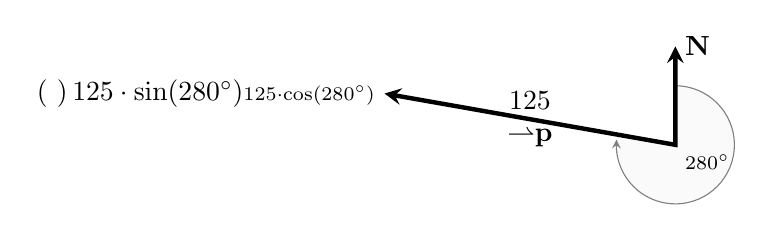
\begin{tikzpicture}[scale=2.5]
      \filldraw[fill=black!2!white,draw=none]
      (0,0) -- (0mm,3mm) arc (90:-190:3mm) -- (0,0);

      \draw[draw=white!50!black,->]
      (0mm,3mm) arc (90:-185:3mm);

      \draw[<->,ultra thick] ({1.5*sin(280)},{1.5*cos(280)}) -- (0,0) -- (0,.5);

      \node[below right] at (0,0) {$\scriptstyle 280^\circ$};
      \node[right] at (0,.5) {\bf N};
      \node[above]  at ({.75*sin(280)},{.75*cos(280)}) {$125$};
      \node[below]  at ({.75*sin(280)},{.75*cos(280)}) {$\vec{p}$};
      \node[left] at ({1.5*sin(280)},{1.5*cos(280)}) {$\begin{pmatrix}\scriptstyle 125\cdot \sin(280^\circ)\\ \scriptstyle 125 \cdot \cos(280^\circ)\end{pmatrix}$};
    \end{tikzpicture}
  \end{center}



To find the coordinates of the plane after it has traveled for $3$
hours, we use $3$ as a scalar to write (round to two decimal places).
\begin{align*}
  3\vec{p} &= \begin{pmatrix}\answer[given]{375}\cdot \sin(280^\circ)\\ \answer[given]{375} \cdot \cos(280^\circ)\end{pmatrix}\\
  &= \begin{pmatrix}\answer[given]{-369.30}\\ \answer[given]{65.12} \end{pmatrix}\\
\end{align*}
\item Now supposing that the wind is blowing at $35$ knots in the true
  bearing of $110^\circ$, we have something like this:
  \begin{center}
    %% A schematic diagram showing a vector at a 330 degree angle with a
    %% vertical line, made in a clockwise fashion. The vectors' length is labeled 125
    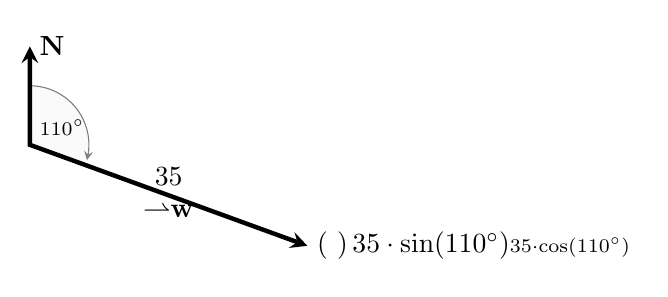
\begin{tikzpicture}[scale=2.5]
      \filldraw[fill=black!2!white,draw=none]
      (0,0) -- (0mm,3mm) arc (90:-20:3mm) -- (0,0);

      \draw[draw=white!50!black,->]
      (0mm,3mm) arc (90:-15:3mm);

      \draw[<->,ultra thick] ({1.5*sin(110)},{1.5*cos(110)}) -- (0,0) -- (0,.5);

      \node[above right] at (0,0) {$\scriptstyle 110^\circ$};
      \node[right] at (0,.5) {\bf N};
      \node[above]  at ({.75*sin(110)},{.75*cos(110)}) {$35$};
      \node[below]  at ({.75*sin(110)},{.75*cos(110)}) {$\vec w$};
      \node[right] at ({1.5*sin(110)},{1.5*cos(110)}) {$\begin{pmatrix}\scriptstyle 35\cdot \sin(110^\circ)\\ \scriptstyle 35 \cdot \cos(110^\circ)\end{pmatrix}$};

    \end{tikzpicture}
  \end{center}
  So now we can solve our problem by computing (round to two decimal places):
  \[
  3\vec{p} + 3 \vec{w} = \begin{pmatrix} \answer[given]{-369.3}\\ \answer[given]{65.12} \end{pmatrix} + \begin{pmatrix} \answer[given]{32.89} \\
  \answer[given]{-11.97} \end{pmatrix} = \begin{pmatrix} \answer[given]{-336.41} \\ \answer[given]{53.15}\end{pmatrix}
  \]
\end{enumerate}
\end{explanation}
\end{example}







\section{The dot product}


We have covered how to add and subtract vectors to get other vectors:
\[
\mathbf{vector} +\mathbf{vector} = \mathbf{vector}
\]
and how to multiply vectors by scalars to get other vectors:
\[
\mathbf{scalar}\cdot \mathbf{vector} = \mathbf{vector}.
\]

However, we \textbf{cannot directly multiply vectors of the same type}.
%% \begin{warning}
%%   There is no general way to ``multiply'' vectors of the same type and
%%   have the resulting product be a reasonable vector also of that type.
%%   You might think it is reasonable to define
%%   \begin{center}
%%     \begin{tikzpicture}
%%       \node at (0,0) {
%%         $\begin{pmatrix}
%%           a_1\\
%%           a_2\\
%%           \vdots\\
%%           a_n
%%         \end{pmatrix}
%%         \cdot
%%         \begin{pmatrix}
%%           b_1\\
%%           b_2\\
%%           \vdots\\
%%           b_n
%%         \end{pmatrix}
%%         =
%%         \begin{pmatrix}
%%           a_1b_1\\
%%           a_2b_2\\
%%           \vdots\\
%%           a_nb_n
%%         \end{pmatrix}$};
%%       \draw[red, line width=5pt,opacity=.3] (-2,-1) -- (2,1);
%%       \draw[red, line width=5pt,opacity=.3] (-2,1) -- (2,-1);
%%     \end{tikzpicture}
%%   \end{center}
%%   but this operation is not especially useful, and will \textbf{never be
%%     utilized in this course}.
%% \end{warning}
%% TK: How about we modify the warning above to something like this? BS: Agreed!
\begin{warning}
  A naive approach to formulation the notion of ``multiplying'' two
  vectors of the same type to produce another vector of that type is
  to define a product via element-by-element multiplication:
  \begin{center}
    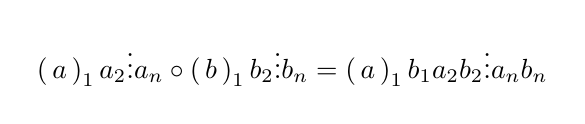
\begin{tikzpicture}
      \node at (0,0) {
        $\begin{pmatrix}
          a_1\\
          a_2\\
          \vdots\\
          a_n
        \end{pmatrix}
        \circ
        \begin{pmatrix}
          b_1\\
          b_2\\
          \vdots\\
          b_n
        \end{pmatrix}
        =
        \begin{pmatrix}
          a_1b_1\\
          a_2b_2\\
          \vdots\\
          a_nb_n
        \end{pmatrix}$};
      % \draw[red, line width=5pt,opacity=.3] (-2,-1) -- (2,1);
      % \draw[red, line width=5pt,opacity=.3] (-2,1) -- (2,-1);
    \end{tikzpicture}
  \end{center}
  This operation is called the \link[\dfn{Hadamard
    product}]{https://en.wikipedia.org/wiki/Hadamard_product_(matrices)},
  and it is used in many interesting applications such as image
  processing and machine learning. For that matter, many numerical
  programming languages natively supports this operation. However, the
  mathematical details about the Hadamard product are slightly beyond
  the scope of this book, and \textbf{will not be discussed any further}.
\end{warning}
 Instead, to ``multiply'' vectors, we use the \textit{dot product}.
 \begin{definition}
  The \dfn{dot product} of two vectors is given by the following.
  \begin{align*}
  \begin{pmatrix}
    a_1\\
    a_2\\
    \vdots\\
    a_n
  \end{pmatrix}
  \dotp
  \begin{pmatrix}
    b_1\\
    b_2\\
    \vdots\\
    b_n
  \end{pmatrix}
  &=\begin{pmatrix} a_1 & a_2 & \cdots & a_n\end{pmatrix}\dotp\begin{pmatrix} b_1 & b_2 & \cdots & b_n\end{pmatrix}\\
  &= \sum_{i=1}^n a_ib_i\\
  &= a_1b_1 + a_2b_2 +\dots+a_nb_n
  \end{align*}
\end{definition}

The first thing you should notice about the the dot product is that
\[
\mathbf{vector}\dotp \mathbf{vector} = \mathbf{number}.
\]


\begin{question}
  Which of the following are vectors?
  \begin{selectAll}
    \pdfOnly{\begin{multicols}{2}}
    \choice[correct]{$(\vec{w} \dotp \vec{u} ) \vec{u}$}
    \choice{$5(\vec{u} +\vec{w}) \dotp {\vec{u}}$}
    \choice{$(2,3) \dotp (4,2) + 7$}
    \choice[correct]{$\vec{w} / ( \vec{u} \dotp \vec{u})$}
    \pdfOnly{\end{multicols}}
    \end{selectAll}
\end{question}


\begin{question}
  Compute:
  \[
  \begin{pmatrix}1 & 2 & 3\end{pmatrix}\dotp\begin{pmatrix}4 & 5 & 6\end{pmatrix}
  \begin{prompt}
    = \answer{32}
  \end{prompt}
  \]
\end{question}







\subsection{Sums via dot product}

The dot product allows us to express sums elegantly in the language of
vectors. For example, the sum of squared terms

\begin{align*}
  \sum_{i=1}^n a_i^2
  & = a_1^2 + a_2^2 + \cdots + a_n^2 \\
  & =
  \underbrace{
    \begin{pmatrix}
      a_1 \\ a_2 \\ \vdots \\ a_n
  \end{pmatrix}}_{=\vec{a}}
  \dotp
  \underbrace{
    \begin{pmatrix}
        a_1 \\ a_2 \\ \vdots \\ a_n
  \end{pmatrix}}_{=\vec{a}} \\
  &= \vec{a} \dotp \vec{a}.
\end{align*}

A sum of multiple terms, $a_1 + a_2 + \cdots + a_n$, can also be
viewed as a dot product:
  \begin{align*}
    \sum_{i=1}^n a_i
    & = 1 \cdot a_1 + 1 \cdot a_2 + \cdots + 1 \cdot a_n \\
    & =
      \underbrace{
      \begin{pmatrix}
        1 \\ 1 \\ \vdots \\ 1
      \end{pmatrix}}_{=\vec{1}}
      \dotp
      \underbrace{
      \begin{pmatrix}
        a_1 \\ a_2 \\ \vdots \\ a_n
      \end{pmatrix}}_{=\vec{a}} \\
      &= \vec{1} \dotp \vec{a}.
  \end{align*}
  The notation $\vec{1}$ denotes the column vector all whose entries
  are ones. This notation will be used throughout the rest of this
  book. In fact the \dfn{mean}, represented by $\mu$, of the entries of the
  $n$-vector $\vec{a}$ can also be described using the dot product as
  \[
  \mu = \frac{\vec{1}\dotp\vec{a}}{n}
  \]

\begin{example}[Finding Averages]
  Suppose that a student's homework scores (in percentage) for a
  linear algebra class are encoded in a column vector $\vec{s}$:
  \[
    \vec{s} =
    \begin{pmatrix}
      90 \\ 85 \\ 100 \\ 80
    \end{pmatrix}
    \qquad
    \begin{array}{l}
      \text{Homework 1}\\
      \text{Homework 2}\\
      \text{Homework 3}\\
      \text{Homework 4}
    \end{array}
    \]
    Use the dot product to compute help compute the average, $\mu$, of
    these scores.
  \begin{explanation}
   Since we can simply dot our vector with the vector $\vec{1}$ to sum
   the data, the average can be expressed by
    \begin{align*}
      \mu
      & = \frac{\vec{1} \dotp \vec{s}}{\answer[given]{4}}\\
      &=\answer[given]{88.75}
    \end{align*}
  \end{explanation}
\end{example}






We summarize the arithmetic and algebraic properties of the dot
product below.
\begin{theorem}
  The following are true for all scalars $s$ and vectors
  $\vec{u}$, $\vec{v}$, and $\vec{w}$ in $\R^n$.
  \begin{description}
  \item[Commutativity:] $\vec{v} \dotp \vec{w} = \vec{w} \dotp
    \vec{v}$
  \item[Linear in first argument:] $(\vec{u}+\vec{v})\dotp \vec{w} = \vec{u}\dotp \vec{w} +
    \vec{v}\dotp \vec{w}$ and $(s\vec{v})\dotp \vec{w} = s(\vec{v}
    \dotp \vec{w})$
  \item[Linear in second argument:] $\vec{u} \dotp (\vec{v}+\vec{w}) = \vec{u}\dotp \vec{v}+
    \vec{u}\dotp \vec{w}$ and $\vec{v} \dotp (s\vec{w}) = s(\vec{v}
    \dotp \vec{w})$
  %\item[Relation to norm:] $\vec{v} \dotp \vec{v} = \|\vec{v}\|^2$
  %\item[Relation to orthogonality:] If $\vec{v}$ is orthogonal to
  %  $\vec{w}$ then $\vec{v} \dotp \vec{w} = 0$.
  \end{description}
\end{theorem}

Instead of defining the dot product by a formula, we could have
defined it by the properties above!  While this is common practice in
mathematics, the process is a bit abstract and is perhaps beyond the
scope of this course.





%% SEE PAGE 25 of notes

\section{Normalizing data}

In many cases, it is useful to to scale data to aid in visualization
and comparison. This process is called
\textit{normalization}. However, it can take different forms depending
on the context. Moreover, the norm allows us to assign a
\textbf{single number to a vector}. In many ways, the idea of taking
something complicated, and reducing it to a single number, is the
heart of mathematics.\index{heart of mathematics}



\subsection{Unit vector normalization, the Euclidean norm}

This involves scaling the vector so that its length (or Euclidean
norm) is $1$. The Euclidean norm of a vector \(\vec{v} = (v_1, v_2,
\ldots, v_n)\) is given by:
\[
\|\vec{v}\| = \sqrt{v_1^2 + v_2^2 + \cdots + v_n^2}
\]
Note that
\[
\|\vec{v}\| = \sqrt{\vec{v}\dotp\vec{v}}.
\]
\begin{definition}
  We call a vector $\hat{\vec u}$ a \dfn{unit vector} if
  \[
  \hat{\vec u} \dotp \hat{\vec u} =1
  \]
  Unit vectors are typically decorated with ``hats.'' Note, this
  necessarily means that $\|\hat{\vec{u}}\| = 1$
\end{definition}



To normalize any vector to a unit vector, we simply divide the vector
by its norm:
\[
\hat{\vec{v}} = \frac{\vec{v}}{\|\vec{v}\|}
\]
now, $\hat{\vec{v}}$ has Euclidean length $1$.

\begin{example}[RGB Color Space]
  Recall that the \textit{MOOCulus Lighting Company} produces an color-changing LED table lamp, whose colors run through the RGB spectrum
    \[
    \underset{\text{red}}{\begin{pmatrix}255\\0\\0\end{pmatrix}},
    \underset{\text{yellow}}{\begin{pmatrix}255\\255\\0\end{pmatrix}},
    \underset{\text{green}}{\begin{pmatrix}0\\255\\0\end{pmatrix}},
    \underset{\text{cyan}}{\begin{pmatrix}0\\255\\255\end{pmatrix}},
    \underset{\text{blue}}{\begin{pmatrix}0\\0\\255\end{pmatrix}},
    \underset{\text{magenta}}{\begin{pmatrix}255\\0\\255\end{pmatrix}}
    \]
    changing colors linearly every minute. However, after consumer
    reviews, it is discovered that the lamp suffers from a small flaw:
    As the colors change, their intensity changes too. In particular,
    yellow, cyan, and magenta, all seem much brighter than red, blue
    and green. Normalize the intensities of the colors so that the
    intensity is constant.
    \begin{explanation}
      To start, we should point out that this is a difficult problem;
      however what we will present is a ``reasonable start'' to
      solution.  Our plan is to normalize the vectors representing
      yellow, cyan, and magenta by their Euclidean norm, then make
      these vectors, unit vectors, then scale back to RGB color space,
      where the entries are between $0$ and $255$. First note:
   \[
   \underset{\vec{y}}{\left\|\begin{pmatrix}255\\255\\0\end{pmatrix}\right\|} =  \underset{\vec{c}}{\left\|\begin{pmatrix}0\\255\\255\end{pmatrix}\right\|} =  \underset{\vec{m}}{\left\|\begin{pmatrix}255\\0\\255\end{pmatrix}\right\|} = \answer[given]{360.624}
   \]
   Naming the vectors above $\vec{y}$, $\vec{c}$, $\vec{m}$, we can find unit vectors
   \begin{align*}
     \hat{\vec y} &= \begin{pmatrix}\answer[given]{181}\\\answer[given]{181}\\\answer[given]{0}\end{pmatrix}\\
     \hat{\vec c} &= \begin{pmatrix}\answer[given]{0}\\\answer[given]{181}\\\answer[given]{181}\end{pmatrix}\\
     \hat{\vec m} &= \begin{pmatrix}\answer[given]{181}\\\answer[given]{0}\\\answer[given]{181}\end{pmatrix}
   \end{align*}
    Here are the actual new colors:
    \begin{center}
      
\begin{tikzpicture}
        \definecolor{rgbyellow}{RGB}{181,181,0}
        \definecolor{rgbcyan}{RGB}{0,181,181}
        \definecolor{rgbmagenta}{RGB}{181,0,181}
        \draw[draw=none,fill={rgb:red,1;green,0;blue,0}] (0,0) rectangle (1,1);
        \draw[draw=none,fill=rgbyellow] (1,0) rectangle (2,1);
        \draw[draw=none,fill={rgb:red,0;green,1;blue,0}] (2,0) rectangle (3,1);
        \draw[draw=none,fill=rgbcyan] (3,0) rectangle (4,1);
        \draw[draw=none,fill={rgb:red,0;green,0;blue,1}] (4,0) rectangle (5,1);
        \draw[draw=none,fill=rgbmagenta] (5,0) rectangle (6,1);
      \end{tikzpicture}
    \end{center}
    Note, this solution can be refined further. In the real world,
    engineers and artist ``tweak'' these colors to actually achieve a
    uniform perception for the human eye.
  \end{explanation}
\end{example}




Given two \textbf{unit} vectors, say $\hat{\vec v}$ and $\hat{\vec w}$, the dot
product measures ``how aligned'' these two unit vectors are.
\begin{description}
  \item[$\hat{\vec{v}}\dotp \hat{\vec{w}} = 1$] If the dot product is $1$, then the vectors are ``completely
    aligned.''
  \item[$\hat{\vec{v}}\dotp \hat{\vec{w}} = -1$] If the dot
    product is $-1$ number, then the vectors are in ``exact opposite''
    directions.
  \item[$\hat{\vec{v}}\dotp \hat{\vec{w}} = 0$]If the dot
    product is zero, then the vectors are independent of each other.
\end{description}


\begin{definition}
  Two vectors are called \dfn{orthogonal} if the the dot product of
  these vectors is zero.
\end{definition}


\begin{question}
  Compute:
  \[
  \begin{pmatrix}1\\1\\-1\end{pmatrix}\dotp\begin{pmatrix}1\\1\\2\end{pmatrix}
  \begin{prompt}
    = \answer{0}
  \end{prompt}
  \]
\end{question}
 When the dot product is zero, we say the vectors are
 \textit{orthogonal} to each other.


As we will see, the notion of orthogonal vectors will allow help us analyze data.






\subsection{Relative component normalization, the $1$-norm}

For comparing relative components, you can normalize a vector by
dividing each component by the absolute value of the sum of all
components. This method ensures that the sum of the vector components
is $1$.

\[ \|\vec{v}\|_1 = \frac{\vec{v}}{\sum_{i=1}^n |v_i|} \]

\begin{example}[Population Counts]
Consider the population vector for Ohio:
\[ \vec{p}_{\texttt{OH}} = (9394878, 1442655, 20442, 268527, 3907, 544866) \]

The sum of the components is:
\[
\vec{1}\dotp\vec{p}_{\texttt{OH}} = \answer[given]{11675275}
\]

The normalized vector is:
\[
\|\vec{p}_{\texttt{OH}}\|_1 =
\frac{\vec{p}_{\texttt{OH}}}{\vec{1}\dotp\vec{p}_{\texttt{OH}}} = \left(\answer[given]{0.8}, \answer[given]{0.12}, \answer[given]{0}, \answer[given]{0.02}, \answer[given]{0}, \answer[given]{0.05}\right)
\]
\end{example}






\subsection{Max component normalization, the $\infty$-norm}

This method involves dividing each component of the vector by the maximum component value. This is useful in cases where you want all components to be scaled relative to the largest component.

\[ \|\vec{v}\|_\infty = \frac{\vec{v}}{\max(|v_i|)} \]

\begin{example}[Student Data]
Suppose the range of score in a certain math class are between $51$
percent and $92$ percent. It is reasonable to use the maximum component
normalization in this case, and scale by $100$ at the end. What is the
range of score after normalizing?
\begin{explanation}
The maximum component is $\answer[given]{92}$. Normalizing we find a
range of $\answer[given]{51/92}$ to $1$. Rescaling so that the maximum
score is $100$, we find the minimum score to be $\answer[given]{55}\%$.
\end{explanation}
\end{example}



\subsection{Which do I use?}
Different normalization techniques are used based on the context and
the specific property you want to normalize for. In demographic
comparisons, relative component normalization ensures that you can
compare proportions directly. For the LED lamp color intensity
normalization, unit vector normalization (Euclidean norm) is
appropriate to ensure consistent intensity across different colors.


%% The dot product allows us to write some complicated formulas quite
%% simply.

%% \begin{definition}
%%   The \dfn{norm} (or magnitude) of vector $\vec{v}$ is given by
%%   \[
%%   \|\vec{v}\|=\sqrt{\vec{v}\dotp\vec{v}}
%%   \]
%% \end{definition}

%% \begin{question}
%%   Compute the norm of the vector $\vec{v} = (1,2,3,4)$.
%%   \begin{prompt}
%%     \[
%%     \|\vec{v}\| = \answer{\sqrt{30}}
%%     \]
%%   \end{prompt}
%% \end{question}
%% When working with a $2$-vector whose entires are real numbers, say
%% $\vec{v} = (x,y)$, we can intepret this data as ``displacement from
%% the origin.''
%% \begin{center}
%%   \begin{tikzpicture}
%%   \draw[->] (-1,0) -- (4,0);
%%   \draw[->] (0,-1) -- (0,3);
%%   \draw[->,ultra thick,penColor] (0,0) -- (3,2);
%%   \node[below right,penColor] at (1.5,1) {$\vec{v}$}; %% <c,d>
%%   \node[right,penColor] at (3,2) {$(x,y)$}; %% <c,d>
%% \end{tikzpicture}
%% \end{center}
%% We can use the distance formula to find the displacement given by
%% $\vec{v}$. Write:
%% \begin{align*}
%%   d &= \sqrt{\left(x-0\right)^{2} + \left(y-0\right)^{2}}\\
%%   &= \sqrt{x^{2} + y^{2}}
%% \end{align*}
%% But this last line is equal to:
%% \begin{align*}
%%   &= \sqrt{\vec{v}\dotp\vec{v}}\\
%%   &= \|\vec{v}\|
%% \end{align*}
%% Hence we see that if we have a $2$-vector $\vec{v}$ (in fact any
%% $n$-vector) whose entires are real numbers, we can intepret
%% \[
%% \|\vec{v}\| = \text{The geometric displacement}
%% \]
%% or ``Euclidean length'' of this vector.
%%  This concept allows us to
%% ``normalize'' vectors and hence data in general.


%% \begin{definition}
%%   A vector $\vec{u}$ is called a \dfn{unit vector} if
%%   \[
%%   \|\vec{u}\| = 1
%%   \]
%% \end{definition}

\end{document}
